\documentclass[default]{beamer}
\setbeamertemplate{navigation symbols}{}

\usetheme{Frankfurt}
%\useoutertheme{infolines}
\usecolortheme{beaver}

\usepackage[utf8]{inputenc}					% Выбор языка и кодировки
\usepackage[english, russian]{babel}	% Языки: русский, английский
\usepackage{csquotes}
\usepackage{tikz}
\usetikzlibrary{arrows,shapes,calc}
\usepackage{animate}
\usepackage{fp}
\usepackage{textpos}
\usepackage{multimedia}
\usepackage{media9}
\usepackage{listings}
\usepackage{minted}

\graphicspath{{../../images/}} 			% Пути к изображениям

\makeatletter
\setbeamertemplate{footline}
{
	\leavevmode%
	\hbox{%
		\begin{beamercolorbox}[wd=.333333\paperwidth,ht=2.25ex,dp=1ex,center]{author
				in head/foot}%
			\usebeamerfont{author in
				head/foot}\insertshortauthor~~\beamer@ifempty{\insertshortinstitute}{}{(\insertshortinstitute)}
		\end{beamercolorbox}%
		\begin{beamercolorbox}[wd=.333333\paperwidth,ht=2.25ex,dp=1ex,center]{title in
				head/foot}%
			\usebeamerfont{title in head/foot}\insertshorttitle
		\end{beamercolorbox}%
		\begin{beamercolorbox}[wd=.333333\paperwidth,ht=2.25ex,dp=1ex,right]{date in
				head/foot}%
			\usebeamerfont{date in head/foot}\insertshortdate{}\hspace*{2em}
			\insertframenumber{}\hspace*{2ex} 
		\end{beamercolorbox}
	}%
	\vskip0pt%
}


\begin{document}
	
	\title[РобоНИС]{НИС: методы искусственного интеллекта в робототехнике}
	\author[Панов, Яковлев]{\textbf{Александр Панов и Константин Яковлев}}
	\institute[ВШЭ]{НИУ ВШЭ}
	\date{18 сентября 2017} 
	
	{
	\setbeamertemplate{headline}{}
	\begin{frame}
		
		\titlepage
		\centering
		\href{mailto:apanov@hse.ru}{apanov@hse.ru}
		
		
\includegraphics[width=25pt]{misc/logos/hse.png} \hspace{10pt}
		\includegraphics[width=100pt]{misc/logos/ras.png} \hspace{10pt}
		
\includegraphics[width=80pt]{misc/logos/frccsc.png}
		
	\end{frame}
	}	

	\section{Введение}
	\subsection{1}
	\begin{frame}
		\frametitle{Кратко о себе}
		\scriptsize
		\begin{columns}
			\begin{column}{0.85\textwidth}
				\textbf{Панов Александр Игоревич, к. ф.-м. н.}
				\begin{itemize}
					\item Старший научный сотрудник лаборатории <<Динамические интеллектуальные системы>> ИСА ФИЦ ИУ РАН.
					\item Научный сотрудник и доцент ФКН ВШЭ.
					\item Доцент кафедры системных исследований Московского физико-технического института (МФТИ).
					\item Член Российской ассоциации искусственного интеллекта (РААИ).
					\item Член Сообщества биологически инспирированных когнитивных архитектур (BICA Society).
					\item Организатор Международной конференции по биологически инспирированным когнитивным архитектурам (BICA-2016 --- Нью-Йорк, BICA-2017 --- Москва), Международной школы по биологически инспирированным когнитивным архитектурам (Fierces on BICA, Москва) и школы молодых ученых по ИИ (ISyT 2017, Санкт-Петербург).
					\item Член редколлегии журнала Biologically Inspired Cognitive Architectures.					
					\item Руководитель проектов РФФИ мол\_а, мол\_а\_дк, офи\_м.
					\item Ментор студенческой лаборатории по ИИ (SLabAI).
				\end{itemize}
			\end{column}
			
			\begin{column}{0.15\textwidth}
				\centering
				\includegraphics[width=\textwidth]{misc/logos/ras.png}
				\vspace{7pt}
				
\includegraphics[width=\textwidth]{misc/logos/frccsc.png}
				\vspace{7pt}
				\includegraphics[width=0.7\textwidth]{misc/logos/isa.png}
				\vspace{7pt}
				\includegraphics[width=0.5\textwidth]{misc/logos/raai.png}
				\vspace{7pt}
				
\includegraphics[width=0.5\textwidth]{misc/logos/hse.png}
				\vspace{7pt}
				\includegraphics[width=\textwidth]{misc/logos/mipt.jpg}
				\vspace{5pt}
				\includegraphics[width=\textwidth]{misc/logos/BICA.png}
				\vspace{5pt}
				\includegraphics[width=0.7\textwidth]{misc/logos/slabai3.png}
			\end{column}
			
		\end{columns}
	\end{frame}

	\begin{frame}
		\frametitle{Техническое}
		
		\centering
		\includegraphics[width=0.9\textwidth]{misc/robots/schedule.png}
		
		\par\bigskip
		
		Обсуждение, вопросы, презентации и ДЗ - на странице курса на Piazza piazza.com/hse.ru/fall2017/aicognitive004
		
	\end{frame}
	

	
	\subsection{Управление роботом}
	\begin{frame}
		\frametitle{Пример: iCub}
		
		
		\begin{columns}
			\begin{column}{0.5\textwidth}
				\centering
				\includegraphics[width=0.8\textwidth]{misc/robots/icub1.jpg}
			\end{column}
			\begin{column}{0.5\textwidth}
				\centering
				\includegraphics[width=0.6\textwidth]{misc/robots/icub2.jpg}
			\end{column}
		\end{columns}
		\par\bigskip
		iCub - один из популярных роботов для разработки и исследований в лабораториях (2005-2010)
	\end{frame}

	\begin{frame}
		\frametitle{Пример: Nao}
		
		
		\begin{columns}
			\begin{column}{0.5\textwidth}
				\centering
				\includegraphics[width=0.5\textwidth]{misc/robots/nao1.jpg}
			\end{column}
			\begin{column}{0.5\textwidth}
				\centering
				\includegraphics[width=0.6\textwidth]{misc/robots/nao2.jpg}
			\end{column}
		\end{columns}
		\par\bigskip
		Nao - следующее поколение андроидных роботов от Aldebaran Robotics (2007-н.в.)
	\end{frame}


	\begin{frame}
		\frametitle{Пример: Darwin}
		
		\centering
		\includegraphics[width=0.7\textwidth]{misc/robots/darwin1.jpg}
		\par\bigskip
		Darwin - современный пример учебного робота (2010-н.в.)
	\end{frame}

	\begin{frame}
		\frametitle{Архитектура управления}
		
		\centering
		\includegraphics[width=0.9\textwidth]{misc/robots/icub_arch.jpg}
		
	\end{frame}
		
	\begin{frame}
		\frametitle{ROS: универсальное ПО}
		
		\centering
		\includegraphics[width=0.9\textwidth]{misc/robots/ros1.png}
		
	\end{frame}


	\section{Когнитивные архитектуры}
	\subsection{2.1}
	\begin{frame}	
		\frametitle{Когнитивные архитектуры}


	Когнитивная архитектура - это набор гипотез о конкретных структурах, которые отвечают за мышление и синтез поведения как в биологических, так и в искусственных системах, и о принципах их совместной работы (Institute of Creative Technologies).
	\par\bigskip
	Наиболее распространенные и разработанные архитектуры:
	\begin{itemize}
		\item Soar (State, Operator And Result)-  \textbf{John Laird}, University of Michigan
		\item ACT-R (Adaptive Control of Thought-Rational) - \textbf{John Anderson}, Carnegie Mellon University
		\item CLARION (Connectionist Learning with Adaptive Rule Induction On-line) - \textbf{Ron Sun}, Rensselaer Polytechnic Institute
		\item LIDA (Learning Intelligent Distribution Agent)  -  \textbf{Stan Franklin}, University of Memphis
		\item Spaun (Semantic Pointer Architecture Unified Network) - \textbf{Chris Eliasmith}, University of Waterloo
	\end{itemize}
	\end{frame}

	\begin{frame}
		\frametitle{Soar: пример когнитивной архитектуры}
		
		\centering
		\includegraphics[width=0.9\textwidth]{misc/robots/soar_arch.png}
		
	\end{frame}

	\begin{frame}
		\frametitle{ACT-R: биологическое правдоподобие}
		
		\centering
		\includegraphics[width=0.6\textwidth]{misc/robots/actr_arch.png}
		
	\end{frame}


	\begin{frame}
		\frametitle{Когнитивный цикл}
		
		\centering
		\includegraphics[width=0.9\textwidth]{misc/robots/soar_circle.png}
		
	\end{frame}

	\begin{frame}
		\frametitle{Представление знаний}
		
		\begin{enumerate}
			\item Логика предикатов первого порядка
			\item Аттрибутивная и дескриптивные логики
			\item Темпоральные и пространственные логики
			\item Байесовские графические модели
			\item Системы правил
			\item Системы фреймов
			\item Семантические сети
			\item Семиотические сети
		\end{enumerate}
		
	\end{frame}

	\section{Gym Environment}
	\subsection{3.1}
	\begin{frame}
		\frametitle{Gym: библиотека для работы с агентами}
		
		\centering
		\begin{center}
			\includemedia[
			activate=onclick,
			width=0.5\textwidth,
			addresource=gym2.mp4
			]{\includegraphics{misc/robots/gym1.png}}{gym2.mp4}
		\end{center}
		
		\par\bigskip
		
		Open AI Gym - библиотека для моделирования работы агентов и их обучения \url{https://gym.openai.com}
		\par\bigskip
		
		
		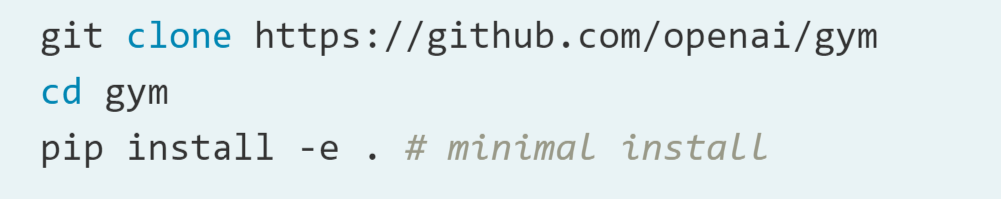
\includegraphics[width=0.6\textwidth]{code1.png}
	\end{frame}
	
	\begin{frame}
		\frametitle{Gym: основной цикл}
		
		\centering
				
		\includegraphics[width=0.4\textwidth]{misc/robots/gym3.png}
		\par\bigskip
		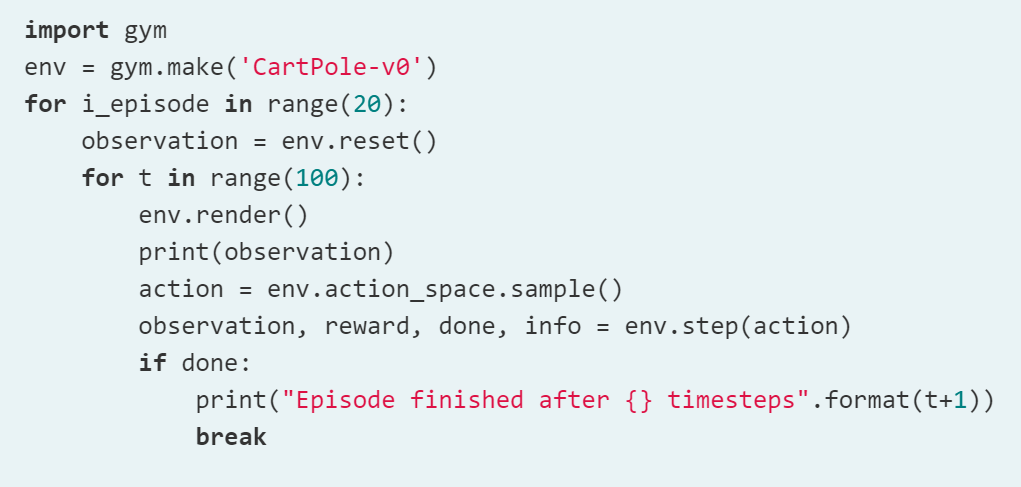
\includegraphics[width=0.7\textwidth]{code2.png}
	\end{frame}	
	
	\begin{frame}
		\frametitle{Задачка поиска пути}
		
		\centering
		
		\includegraphics[width=0.4\textwidth]{examples/path/path_example.png}
		\par\bigskip
		\includegraphics[width=0.7\textwidth]{examples/path/neural_arch.png}
	\end{frame}
	
\end{document}
	
	
